\subsection{Terrain}
Un terrain de Quidditch est délimité par un ovale, et est constitué de cases hexagonales de 10 pieds\footnote{3.048 m}. Il fait 50 cases dans sa plus grande longueur, et 18 cases dans sa plus grande largeur, pour un total de 706 cases sur le terrain.

Chaque case ne peut accueillir qu'un seul joueur au maximum. Si deux joueurs arrivent au même tour sur la même case, une collision a lieu. Selon les \gls{aptitude}s et les rôles des joueurs, différentes actions indirectes pourront avoir lieu.

\subsubsection{Déplacement des joueurs}
\begin{figure}[h!]
    \centering
    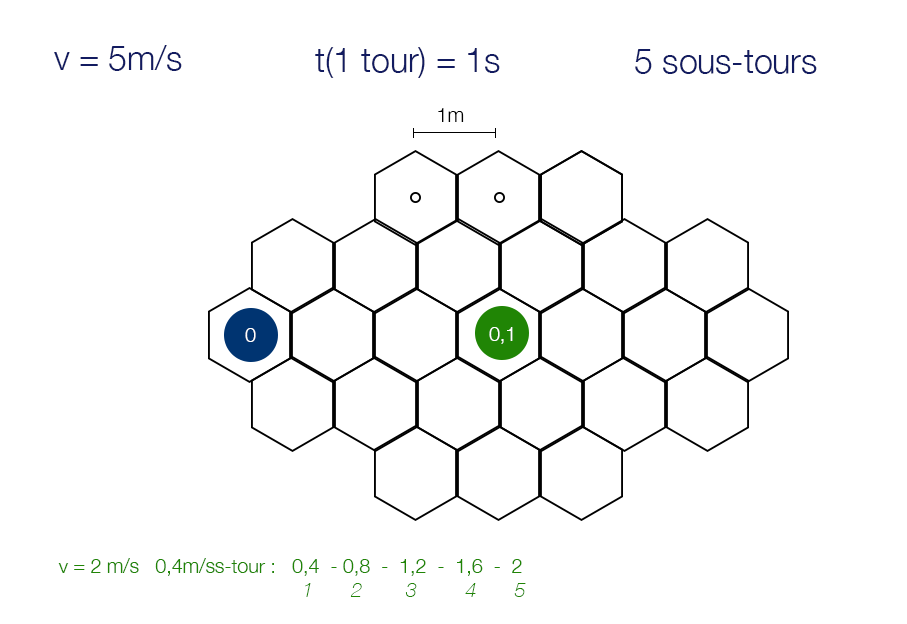
\includegraphics[width=0.3\textwidth]{../TurnModel/TurnModel0.png}
    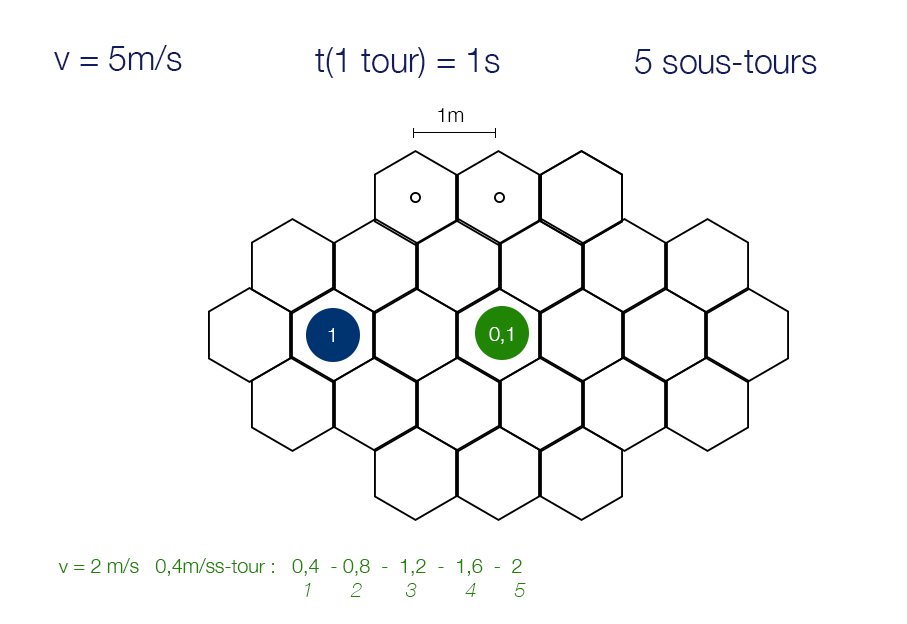
\includegraphics[width=0.3\textwidth]{../TurnModel/TurnModel1.png}
    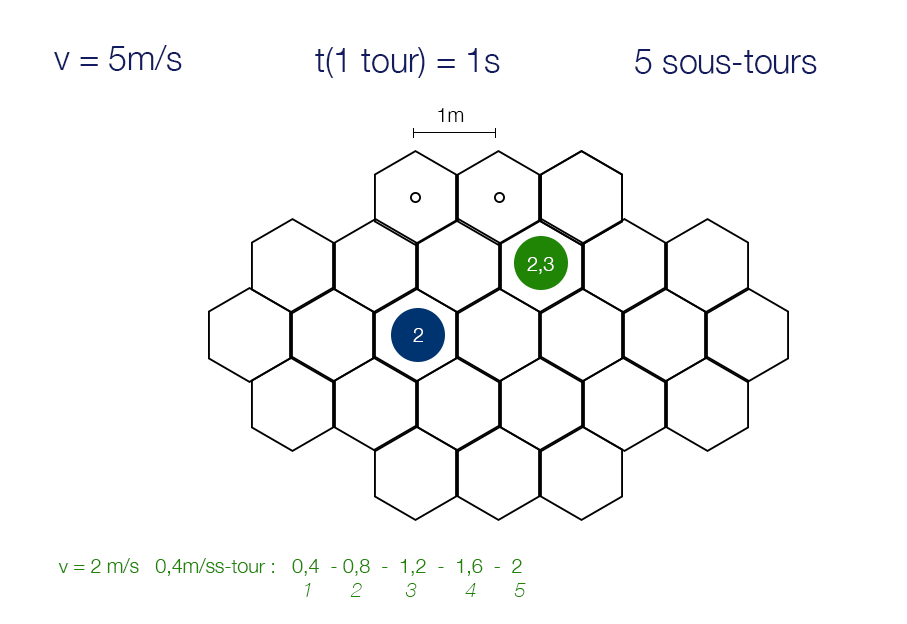
\includegraphics[width=0.3\textwidth]{../TurnModel/TurnModel2.png}
    \\
    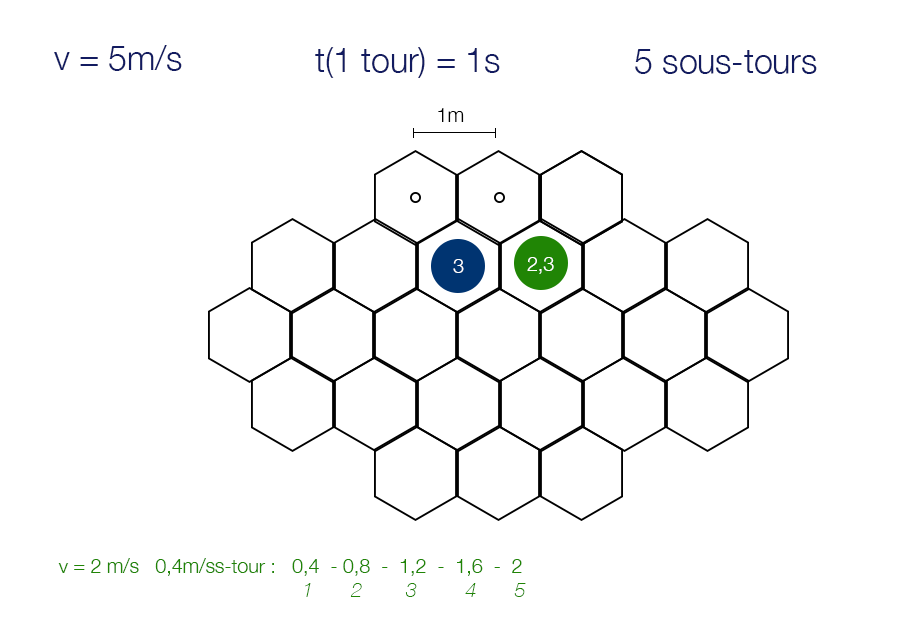
\includegraphics[width=0.3\textwidth]{../TurnModel/TurnModel3.png}
    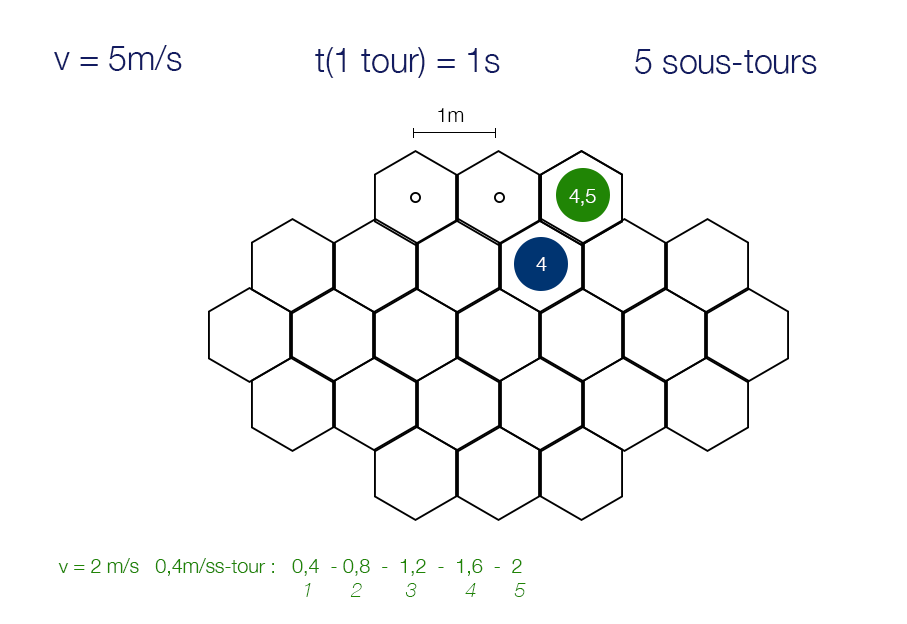
\includegraphics[width=0.3\textwidth]{../TurnModel/TurnModel4.png}
    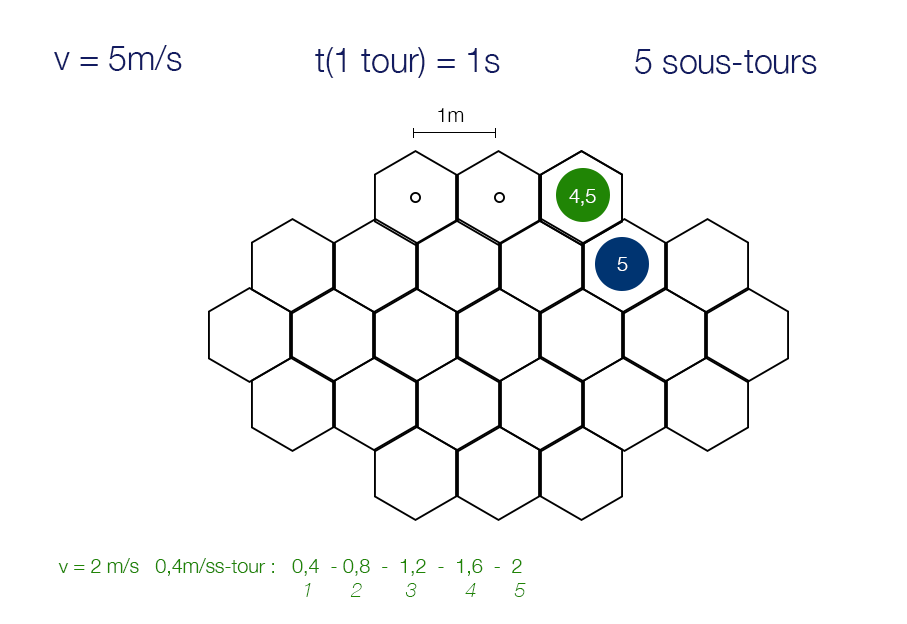
\includegraphics[width=0.3\textwidth]{../TurnModel/TurnModel5.png}
    \caption{\label{fig:TurnModel} Déplacements des joueurs sur le terrain}
\end{figure}

Un tour de jeu est divisé en $n$ intervalles isochroniques, avec $n$ la plus grande vitesse parmis tous les objets déplaçables. La figure \ref{fig:TurnModel} illustre la procédure utilisée. Pour chaque instant, de $t = \frac{1}{n}$ à $t = 1$, pour chaque déplacement à jouer\footnote{Les déplacements sont ordonnés par ordre de réception}, on calcule la position de l'objet déplaçable. Si aucun autre déplaçable ne se trouve à la position calculée, on y place le déplaçable en cours de mouvement. Dans le cas contraire, une collision a lieu.

\subsubsection{Collisions}
Chaque déplaçable a un score de collision, dépendant de ses caractéristiques et d'un jet de dé aléatoire. Lorsqu'une collision a lieu, on demande le score de collision de chacun des déplaçables. Celui ayant le plus grand remporte la case disputée. Plusieurs sous-cas peuvent alors se présenter:

\paragraph{Le premier joueur sur la case gagne}
Le second prétendant à cette position voit son mouvement arrêté. Il es placé sur la dernière case qu'il a atteint et son déplacement est supprimé de la case

\paragraph{Le second arrivant gagne}
Le premier joueur est placé sur une case libre adjacente, son mouvement est supprimé, et le second joueur lui vole la position.

\paragraph{Un des deux déplaçable est attrapable par l'autre}
Le joueur attrape l'autre déplaçable.
